\documentclass{beamer}
	\usepackage[utf8]{inputenc}		% required for umlauts
	\usepackage[ngerman]{babel}		% required for umlauts
	\usepackage[sfdefault]{roboto}	% enable sans serif font roboto
	%\usepackage{libertine}			% enable this on Windows to allow for microtype
	\usepackage[T1]{fontenc}		% required for output of umlauts in PDF

	\usepackage{mathtools}		% required for formulas

	\usepackage{graphicx}		% required to insert images
	\usepackage[space]{grffile} % insert images baring a filename which contains spaces
	\usepackage{float}			% allow to forcefully set the location of an object

	\usepackage[tracking=true]{microtype} % required to change character spacing

	\usepackage{hyperref}		% insert clickable references

	\usepackage{datetime}		% flexible date specification
	\newcommand{\leadingzero}[1]{\ifnum#1<10 0\the#1\else\the#1\fi}
	\newcommand{\todayddmmyyyy}{\leadingzero{\day}.\leadingzero{\month}.\the\year}

	\usepackage{geometry}
	\usepackage{scrextend}		% allow arbitrary indentation

	\usepackage{color}

	\usetheme{default}
	\usecolortheme{beaver}

	\title{First Weekly Update on `Optimization~of~Particle~Identification'}
	\subtitle{ROC curve, $\epsilon_{PID}$-matrix and various statistics}
	\author{Gordian Edenhofer}
	\date{\today}


\begin{document}
\begin{frame}
	\frametitle{Git Log}

	\begin{columns}[T]
		\begin{column}{.5\textwidth}
			\begin{itemize}
				\item Calculate and plot a ROC curve
				\item Compute and visualize an $\epsilon_{PID}$-matrix
				\item Visualize precision and recall
				\item Evaluate various `pid*' variables and reconstruct particleIDs
				\item Construct a naive alternative to the particleID variables using Bayes
			\end{itemize}
		\end{column}
		\begin{column}{.5\textwidth}
			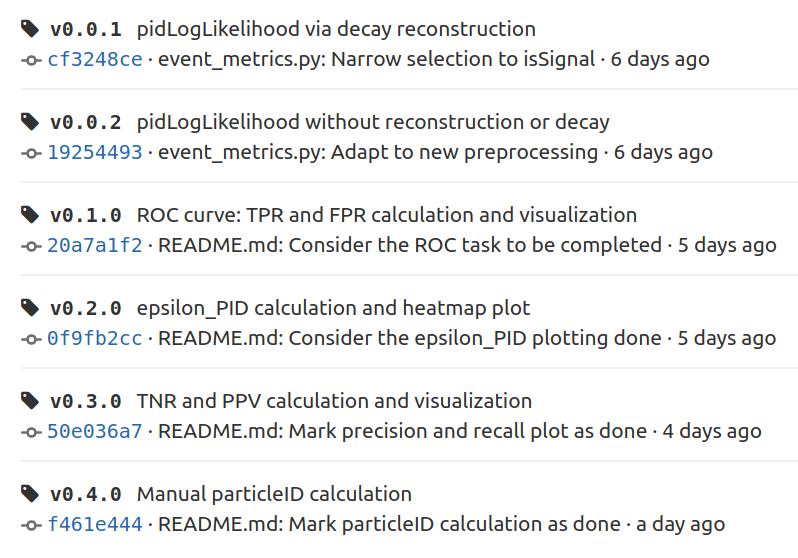
\includegraphics[width=1\linewidth]{res/01-git tags.png}
		\end{column}
	\end{columns}
\end{frame}

\begin{frame}
	\frametitle{Inventory}
	\framesubtitle{ROC-curve, TPR, TNR and PPV}

	Tested Sample Decay: \hspace{2em}
	$B^+ \rightarrow \mu^+ \nu_{\mu}$
	\hspace{2em}
	$B^- \rightarrow \pi^- D^0$
	\\
	\begin{addmargin}[1em]{0em}
		$D^0 \rightarrow K^- \pi^+$ ,
		$D^0 \rightarrow K^- \pi^+ \pi^0$,
		$D^0 \rightarrow K^- \pi^+ \pi^+ \pi^-$,
		$D^0 \rightarrow K^- K^+$,
		$D^0 \rightarrow \pi^+ \pi^0$
	\end{addmargin}

	\vspace{1em}

	\centering
	\includegraphics[height=0.65\textheight]{res/Statistics for K+ identification (via bayes)}
\end{frame}

\begin{frame}
	\frametitle{Inventory}
	\framesubtitle{$\epsilon_{PID}$-matrix}

	\centering
	\includegraphics[height=0.7\textheight]{res/Heatmap of epsilon_PID-matrix (via ID, cut at 0.2).pdf}
\end{frame}

\begin{frame}
	\frametitle{Exploratory (WIP)}
	\framesubtitle{ParticleID Approach in comparison to Bayesian Approach}

	Tested Sample Decay: \hspace{2em}
	$B^+ \rightarrow \mu^+ \nu_{\mu}$
	\hspace{2em}
	$B^- \rightarrow \pi^- D^0$
	\\
	\begin{addmargin}[1em]{0em}
		$D^0 \rightarrow K^- \pi^+$,
		$D^0 \rightarrow K^- \pi^+ \pi^0$,
		$D^0 \rightarrow K^- \pi^+ \pi^+ \pi^-$,
		$D^0 \rightarrow K^- K^+$,
		$D^0 \rightarrow \pi^+ \pi^0$
	\end{addmargin}

	\vspace{1em}

	\begin{columns}[T]
		\begin{column}{.5\textwidth}
			\centering ParticleID Approach
			\includegraphics[width=1\linewidth]{res/Statistics for K+ identification (via bayes)}
		\end{column}
		\begin{column}{.5\textwidth}
			\centering Bayesian Approach
			\includegraphics[width=1\linewidth]{res/Statistics for K+ identification (via bayes).pdf}
		\end{column}
	\end{columns}
\end{frame}

\begin{frame}
	\frametitle{Exploratory (WIP)}
	\framesubtitle{ParticleID Approach in comparison to Bayesian Approach}

	\begin{columns}
		\column{0.5\textwidth}
		\begin{minipage}[c][0.4\textheight][c]{\linewidth}
			\centering
			\includegraphics[width=0.8\linewidth]{res/Statistics for pi+ identification (via ID).pdf}
		\end{minipage}
		\begin{minipage}[c][0.4\textheight][c]{\linewidth}
			\centering
			\includegraphics[width=0.8\linewidth]{res/Statistics for mu+ identification (via ID).pdf}
		\end{minipage}

		\column{0.5\textwidth}
		\begin{minipage}[c][0.4\textheight][c]{\linewidth}
			\centering
			\includegraphics[width=0.8\linewidth]{res/Statistics for pi+ identification (via bayes).pdf}
		\end{minipage}
		\begin{minipage}[c][0.4\textheight][c]{\linewidth}
			\centering
			\includegraphics[width=0.8\linewidth]{res/Statistics for mu+ identification (via bayes).pdf}
		\end{minipage}
	\end{columns}
\end{frame}

\end{document}
